% Metódy inžinierskej práce

\documentclass[10pt,twoside,slovak,a4paper]{article}

\usepackage[slovak]{babel}
%\usepackage[T1]{fontenc}
\usepackage[IL2]{fontenc} % lepšia sadzba písmena Ľ než v T1
\usepackage[utf8]{inputenc}
\usepackage{graphicx}
\usepackage{url} % príkaz \url na formátovanie URL
\usepackage{hyperref} % odkazy v texte budú aktívne (pri niektorých triedach dokumentov spôsobuje posun textu)

\usepackage{cite}
%\usepackage{times}


\title{Vývoj mobilných aplikácií modelom MDE\thanks{Semestrálny projekt v predmete Metódy inžinierskej práce, ak. rok 2021/21, vedenie: Ing. Vladimír Mlynaroviè, PhD.}} % meno a priezvisko vyučujúceho na cvičeniach

\author{Oliver Hofer\\[2pt]
	{\small Slovenská technická univerzita v Bratislave}\\
	{\small Fakulta informatiky a informačných technológií}\\
	{\small \texttt{xhofer@stuba.sk}}
	}

\date{\small 06.november  2021} % upravte



\begin{document}

\maketitle

\begin{abstract}
Cieľom článku bude zamerať sa na vývoj mobilných aplikácií s použitím MDE (Model driven approach). Pri modelovom softvérovom programovaní sa konkrétne zameriam na využite UML na vytváranie diagramov. Tiež by som chcel popísať výhody a nevýhody tohto postupu. Následne si opíšeme rôzne typy diagramov UML, ktoré pri vývoji aplikácií môžeme využívať a následne si ich taktiež porovnáme. V ďalšej časti si popíšeme hlavnú výhodu tejto metódy, čo je generovanie kódu na základe vytvorených diagramov za použitia nástroja GenCode. Na koniec článku v časti ~\ref{zaver},si tento model zhodnotíme a urobíme záver.
\end{abstract}



\section{Úvod}
\cite{2012}
Smartfóny so v dnešnej dobe súčasťou nášho každodenného života. Tieto malé zariadenia často nahrádzajú veľké stolové počítače alebo notebooky. Ešte pred pár rokmi by sme to o týchto zariadeniach povedať nemohli. Zato môžeme ďakovať hlavne vývoju hardvéru a softvéru. \newline
Taktiež za to môžeme ďakovať MDE (Model driven engineering), ktoré veľmi pomáha zefektívňovať písanie kódu. Ako tento spôsob funguje sa dozviete ďalej v článku v časti~\ref{MDE spôsob pre Android}.\newline
Momentálne väčšina zariadení používa systém Android, a preto som sa aj rozhodol sa zamerať v tomto článku konkrétne na tento systém.

\newpage
\section{Myšlienková mapa} \label{Myšlienková mapa}


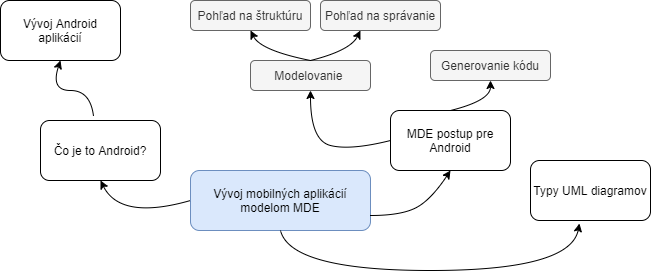
\includegraphics[scale=0.65]{myšlienková mapa.png}


\section{Čo je to Android?} \label{Čo je to Android?}
Android je rozsiahla open-source platforma založená jadre Linuxu. Tento operačný systém je vlastnený spoločnosťou Google. Tento systém bol pôvodne vytvorený pre digitálne fotoaparáty. V dnešnej dobe sa však používa v Mobilných smartfónoch, tabletoch, televíziách, nositeľných zariadeniach, v systémoch v autách... 



\section{Vývoj Android aplikácii } \label{Vývoj Android aplikácii}

Android aplikácie boli v minulosti aj dnes vyvíjané za pomoci jazyku Java.\cite{9032440} Avšak dnes sa začínajú využívať alternatívy ako je Kotlin alebo Dart a mnoho ďalších. Pri písaní programu sa používajú SDK (Software development kit) čo je softvér nástrojov pre vývojárov. IDE (integrated Development Environment) čo je skratka pre integrované vývojové prostredie. \newline
Hlavné vývojové prostredie pre Android aplikácie je Android Studio, ktoré poskytuje flexibilnú platformu pre developerov, kde môžu používať rôzne SDK. Pre jazyky Kotlin a Java sa používa rovnaké SDK ale jazyk Dart používa SDK, ktoré sa volá Flutter. \newline
Súčasťou SDK je väčšinou Dalvik. Dalvik je virtuálny stroj na, ktorom beží operačný systém Android. Využíva sa na rýchle testovanie aplikácií bez potreby pripájať mobilné zariadenie. Tento nástroj tiež veľmi zefektívňuje proces programovanie.\newline
Hlavnou zložkou Android aplikácií je Aktivita. Android aplikácia väčšinou obsahuje jednu alebo viac aktivít. Aktivita sa zobrazuje ako jedno používateľské prostredie, ktoré si vieme predstaviť ako karty s prvkami, s ktorými môže užívateľ pracovať.\newline
Servis je špeciálna aktivita, ktorá nemá užívateľské rozhranie a pracuje na pozadí. Pracujú na aplikačnej rámcovej vrstve (App Framework Layer). Spolu s aktivitou sú to najpoužívanejšie komponenty pri programovaní Android Aplikácií. \newline
Každá aktivita v Android kóde má svoj životný cyklus (lifecycle). Je to vlastnosť aplikácie, ktorá určuje čo sa má s určitou aktivitou diať v určitých prípadoch. Napríklad, čo sa stane s aktivitou keď sa spustí aplikácia alebo čo sa stane s aktivitou keď sa aplikácia stane... 








\section{MDE postup pre Android} \label{MDE spôsob pre Android}

\subsection{Modelovanie}\label{MDE spôsob pre Android:Modelovanie}
Tento spôsob popisuje ako kompletne popísať štruktúru a správanie Android aplikácie použitím štandardu UML. Tento spôsob sa pozerá na konkrétne veci nie na kompletný kód. Pri modelovaní poznáme pohľad na štruktúru a Pohľad na správanie.

\subsubsection{Pohľad na štuktúru}\label{MDE spôsob pre Android:Modelovanie:Pohľad na štuktúru}
afasfasfasfdasfas
afafafaf

\subsubsection{Pohľad na správanie}\label{MDE spôsob pre Android:Modelovanie:Pohľad na správanie}
afasdfasfaf
afaasdfasfa


\subsection{Generovanie kódu}\label{Generovanie kódu}
Hlavným benefitom adaptovania MDE postupu pri vyvíjaní Android aplikácii je automatizácia v podobe generovania kódu. Na generovanie kódu môžeme použiť diagramy tried alebo diagramy postupnosti.\newline
Z diagramu tried program na generovanie vygeneruje základnú aplikačnú štruktúru a súbory v jazyku Java pre každú triedu.\newline
Bohužiaľ generovanie kódu na základe grafov postupnosti má svoje limity. Napríklad jednoduché operácie ako generovanie dynamicky alokovaných polí nesú možné. Avšak dokáže generovať časti kódu ako podmienky a cykly.


\section{Typy UML diagramov} \label{Typy UML diagramov}




\section{Záver} \label{zaver} % prípadne iný variant názvu



%\acknowledgement{Ak niekomu chcete poďakovať\ldots}

\newpage
% týmto sa generuje zoznam literatúry z obsahu súboru literatura.bib podľa toho, na čo sa v článku odkazujete
\bibliography{literatura}
\bibliographystyle{plain} % prípadne alpha, abbrv alebo hociktorý iný
\end{document}
